% begin module first-derivative-test
\begin{frame}
\begin{itemize}
\item  Recall that if $f$ has a local maximum at $c$, then $c$ must be a critical number for $f$, but if $c$ is a critical number for $f$, it is not necessarily a local maximum.
\item<2->  In the first picture, $f'(x) > 0$ to the left of $c$ and $f'(x) < 0$ to the right of $c$.
\item<3->  In other words, $f'(x)$ changes sign at $c$.
\item<4->  In the second picture, $f'(x) > 0$ to the left of $c$ and $f'(x) > 0$ to the right of $c$.  $f'(x)$ doesn't change sign at $c$.
\item<5->  In the first picture there's a local maximum, but not in the second.
\item<6->  This suggests a way of testing for local maxima/minima.
\end{itemize}
\begin{columns}[c]
\column{.5\textwidth}
\ 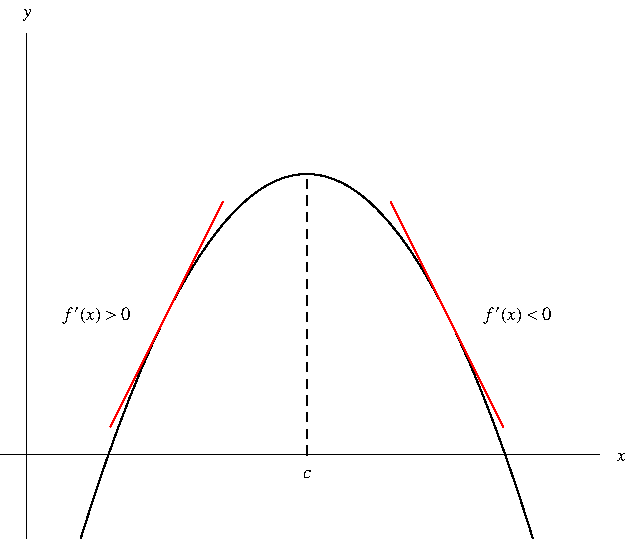
\includegraphics[height=3cm]{curve-sketching/pictures/04-03-firstderiva.pdf}%
\column{.5\textwidth}
\ 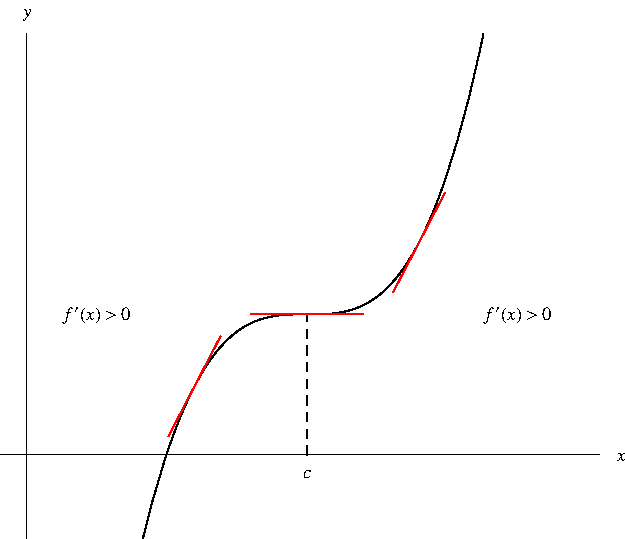
\includegraphics[height=3cm]{curve-sketching/pictures/04-03-firstderivc.pdf}%
\end{columns}
\end{frame}



\begin{frame}
The First Derivative Test

Suppose that $c$ is a critical number of a continuous function $f$.
\begin{enumerate}
\item<1-| alert@2>  \alert<handout:1| 0>{If $f'$ changes from positive to negative at $c$, then $f$ has a local maximum at $c$.}
\item<1-| alert@3>  \alert<handout:2| 0>{If $f'$ changes from negative to positive at $c$, then $f$ has a local minimum at $c$.}
\item<1-| alert@4>  \alert<handout:3| 0>{If $f'$ doesn't change signs at $c$, then $f$ has no local maximum or minimum at $c$.}
\end{enumerate}
\begin{columns}[c]
\column{.5\textwidth}
\ \only<handout:1| -2>{%
\uncover<2>{%
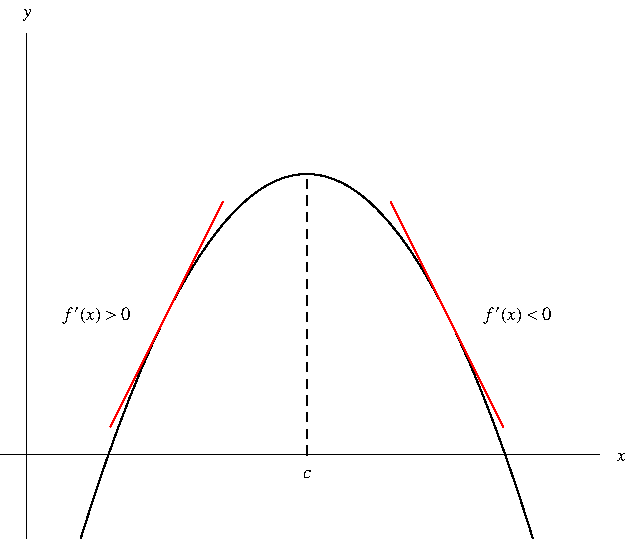
\includegraphics[height=4cm]{curve-sketching/pictures/04-03-firstderiva.pdf}%
}}%
\only<handout:2| 3>{%
\uncover<3>{%
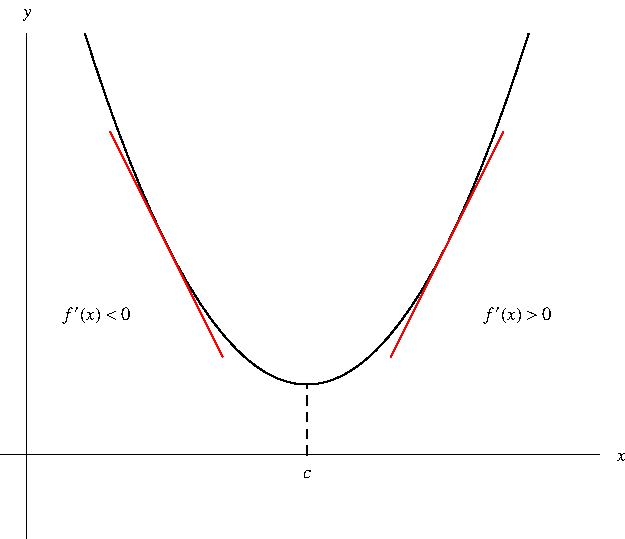
\includegraphics[height=4cm]{curve-sketching/pictures/04-03-firstderivb.pdf}%
}}%
\only<handout:3| 4->{%
\uncover<4->{%
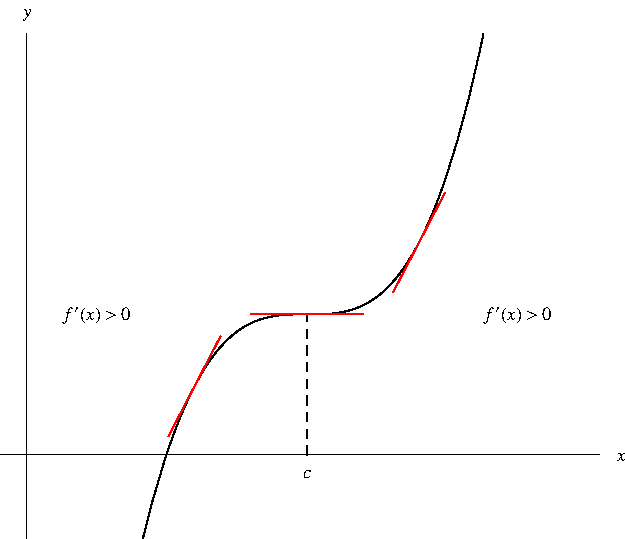
\includegraphics[height=4cm]{curve-sketching/pictures/04-03-firstderivc.pdf}%
}}%
\column{.5\textwidth}
\uncover<handout:3| 4->{%
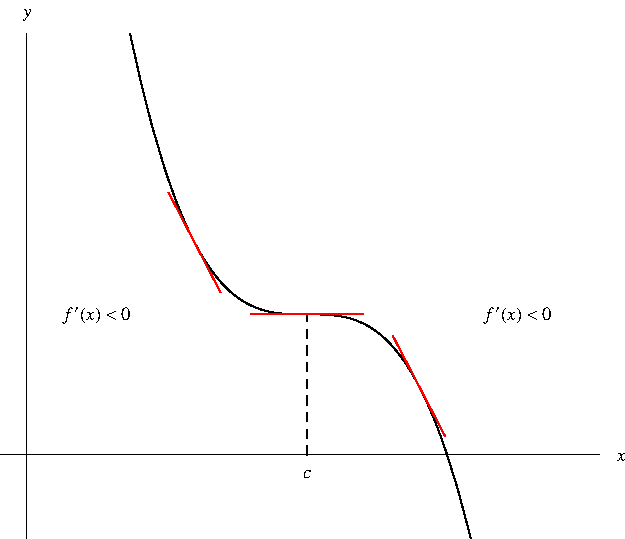
\includegraphics[height=4cm]{curve-sketching/pictures/04-03-firstderivd.pdf}%
}%
\end{columns}
\end{frame}
% end module first-derivative-test
